\documentclass[12pt]{article}
\usepackage{amsmath}
\usepackage[shortlabels]{enumitem}
\usepackage{tcolorbox}

\usepackage{graphicx}
\usepackage{amsthm}
\usepackage{amssymb}
\usepackage{thmtools}
\usepackage{amsthm}
\usepackage{algorithm}
\usepackage{algpseudocode}
\usepackage{xspace}
\usepackage{CJKutf8}
\usepackage[hidelinks,pdfencoding=auto,psdextra]{hyperref}

\usepackage{graphicx}
\usepackage{pythonhighlight}


%\renewcommand{\thepage}{}

\textwidth=6.7in
\textheight=8.4in
\oddsidemargin=-.3in
\evensidemargin=-.1in
\topmargin=-.3in

\newcommand{\Bskip}{\vspace*{.3in}}
\newcommand{\Solution}{\ \\ \textbf{Solution:} }
\newcommand{\Answer}{\ \\ \textbf{Answer:} }
\newtheorem{theorem}{Theorem}
\newtheorem{remark}{Remark}
\newtheorem{hint}{Hint}
\newtheorem{definition}{Definition}

\DeclareMathOperator*{\E}{\mathbb{E}}
\newcommand{\Var}{\mathsf{Var}}
\newcommand{\Cov}{\mathsf{Cov}}
\newcommand{\Covar}{\mathsf{Covar}}
\declaretheoremstyle[headfont=\bf]{normalhead}
\declaretheorem[style=normalhead]{problem}
\def\ie{\textit{i.e.}\xspace}
\def\eg{\textit{e.g.}\xspace}
\newcommand{\Name}{Jin Fang}
\newcommand{\ChineseName}{方缙}

\begin{document}

\noindent
\hspace*{.2in} COMP7102P Fall 2022
\hfill Homework 3\\
\begin{CJK}{UTF8}{gbsn}
    \hspace*{.2in} \textcolor{red}{BA22011024 \Name{} \ChineseName} \hfill due: Oct. 27, 09:30
\end{CJK}
\bigskip


\begin{problem}[30 points] Answer the following questions and show your calculations.
\begin{enumerate}
  \item Compute the stationary distribution of the standard random walk (pick a random outgoing edge and traverse along this edge) for the following directed graph.
  \begin{figure}[H]
    \centering
    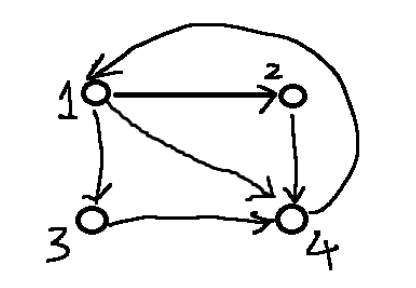
\includegraphics[width=2in]{images/123.png}
  \end{figure}     
  Remark: Unlike undirected graphs whose stationary distributions have a close form, there is no close form for directed graph.
   
  \Answer
  The transition matrix of the above graph is 
  \begin{equation}
  A = { \left( \begin{array}{cccc}
    0 & \frac{1}{3} & \frac{1}{3} & \frac{1}{3}\\
    0 & 0 & 0 & 1\\
    0 & 0 & 0 & 1 \\
    1 & 0 & 0 & 0 \end{array} \right)}
  \end{equation}
 
  Let $\mathbf{\pi} = (\pi_1, \pi_2, \pi_3, \pi_4)$ denote the stationary distribution. Since $\mathbf{\pi} \cdot A = \mathbf{\pi}$, we have:

  \begin{align}\label{eq:1}
  \begin{cases}
  \pi_4 = \pi_1\\
  \frac{\pi_1}{3} = \pi_2\\
    \frac{\pi_1}{3} = \pi_3\\
    \frac{\pi_1}{3}+\pi_2+\pi_3 = \pi_4\\
    \pi_1+ \pi_2+ \pi_3+ \pi_4 =1
  \end{cases}
  \end{align}
 
  By solving Eq .\eqref{eq:1}, we can obtain:

  \begin{align}
  \begin{cases}
    \pi_1 = \frac{3}{8}\\
    \pi_2 = \frac{1}{8}\\
    \pi_3 = \frac{1}{8}\\
    \pi_4 = \frac{3}{8}
  \end{cases}
  \end{align}

  Thus, the stationary distribution is $\mathbf{\pi} = (\frac{3}{8}, \frac{1}{8},\frac{1}{8}, \frac{3}{8})$.
      
  \item Consider a start graph with $n$ vertices. Suppose vertex 1 is the center. What are the hitting time $h_{1,2}$ and $h_{2,1}$?
   \begin{figure}[H]
      \centering
 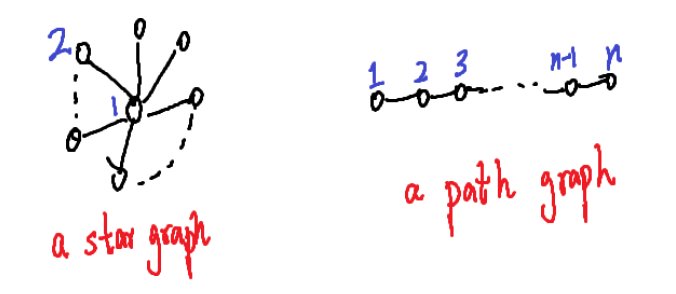
\includegraphics[width=4in]{images/1234.png}
\end{figure} 
  
  \Answer
  
  Obviously, $h_{2,1} = 1$. We then calculate the value of $h_{1,2}$. For a star graph, we have:

  \begin{align}\label{eq:2}
  \begin{cases}
    h_{1,2} = \sum_{i=3}^{n}\frac{1+h_{i,2}}{n-1} + \frac{1}{n-1}\\
    h_{3,2} = 1+h_{1,2}\\
    \cdots\\
    h_{n,2} = 1+h_{1,2}
  \end{cases}
  \end{align}

  According to Eq. \eqref{eq:2}, we can obtain:

  \begin{align}
    & h_{1,2} = \frac{(n-2) \cdot (2+h_{1,2}) + 1}{n-1} \notag\\
   \Rightarrow & h_{1,2} \cdot (n-1) = (n-2) \cdot (2+h_{1,2}) +1 \notag\\
   \Rightarrow &  h_{1,2} = 2 \cdot n-3  
  \end{align}
  
  \item Consider a path graph with from 1 to n. What are the hitting time $h_{1,n}$ and $h_{n,1}$?
  
  \Answer

  For a linear graph, we have

  \begin{align}\label{eq:3}
  \begin{cases}
    h_{1,n} = 1+h_{2,n} \\
    h_{2,n} =1+ \frac{1}{2}(h_{1,n}+h_{3,n})\\
    h_{3,n} =1+ \frac{1}{2}(h_{2,n}+h_{4,n})\\
    h_{4,n} =1+ \frac{1}{2}(h_{3,n}+h_{5,n})\\
    \cdots\\
    h_{n-2,n} =1+ \frac{1}{2}(h_{n-1,n}+h_{n-3,n})\\
    h_{n-1,n} =1+ \frac{1}{2}h_{n-2,n}
  \end{cases}
  \end{align}
  
  By accmulating both sides of Eq. \eqref{eq:3} we get:

  \begin{align}
  &  \frac{h_{1,n}}{2}-\frac{h_{2,n}}{2}+\frac{h_{n-1,n}}{2} = n-1 \notag \\
   \rightarrow &h_{n-1,n} = 2n-3
  \end{align}

  By applying $h_{n-1,n} = 2n-3$ to Eq. \eqref{eq:3} we have:
  
  \begin{align}\label{eq:4}
  \begin{cases}
    h_{n-1,n} = 2n-3 \\
    h_{n-2,n} =4n-8\\
    h_{n-3,n} =6n-15\\
    \cdots\\
    h_{n-i,n} =2 \cdot n \cdot i - i^2 -2 \cdot i\\
    \cdots\\
    h_{2,n} =n(n-2)\\
    h_{1,n} =n(n-2)+1
  \end{cases}
  \end{align}

As a result, we can obtain that $h_{1,n} =(n-1)^2$ and $h_{n,1} =(n-1)^2$.
  
  
\end{enumerate}

\end{problem}

\begin{problem}[40 points] Let us compute the mixing time by a different way. Let $A$ be the transition matrix of a undirected graph $G: A(i, j) = 1/d(i) \text{\ iff\ }(i, j) \in E$. Let $A = \sum_{i=1}^{n}\lambda_i\cdot D^{-1/2}\mathop{v_{i}}\limits ^{\rightarrow}\cdot D^{-1/2}{\mathop{v_{i}}\limits ^{\rightarrow}}^\top$ be its eigen-decomposition where $\mathop{v_{1}}\limits ^{\rightarrow},\mathop{v_{2}}\limits ^{\rightarrow},...,\mathop{v_{n}}\limits ^{\rightarrow}$ constitute an orthonormal basis.
\end{problem}
\begin{enumerate}
	\item Write all facts that we have shown about $\lambda_1,...,\lambda_n$ and $\mathop{u_{1}}\limits^{\rightarrow}$.
	
  \Answer

  \begin{enumerate}[(a)]
      \item $1=\lambda_1 \geq \ldots \geq\lambda_n$.
      \item $\lambda_2 \le 1$ iff $G$ is connected.
      \item $\lambda_n \ge -1$ iff $G$ is not bipartite.
      \item $v_1=\left(\sqrt{\frac{d(1)}{2m}},\ldots, \sqrt{\frac{d(n)}{2m}}\right)^T$.
  \end{enumerate}

  \item Let $p_0$ be the distribution of the starting point of our random walk. Prove $p_t^\top=p_0^\top\cdot A^t$ and $||p_t - \pi||_2 \le \max\{\lambda_2,|\lambda_n|\}\cdot||p_{t-1}-\pi||_2$.
    
  \Answer
  Let $A$ denote the transition matrix, we have $p_1^T=p_0^T \cdot A$ and $p_2^T=p_1^T \cdot A=p_0^T \cdot A^2$. Accordingly, $p_t^T=p_{t-1}^T \cdot A= \ldots =p_0^T \cdot A^t$. Thus, we have:

  \begin{equation}
      p_t(j)=\sum_i^n p_0(i) \cdot A^t(i,j)
  \end{equation}

  Similar to the process in Lec. 4, we have:

  \begin{equation}
      \begin{aligned}
          A^t &= \left(\sum_{k=1}^n \lambda_k \cdot D^{-\frac{1}{2}} \cdot \vec{v_k} \cdot D^{\frac{1}{2}} \cdot \vec{v_k}^T  \right)\\
          &= D^{-\frac{1}{2}} \cdot \left(\sum_{k=1}^n \lambda_k^t \cdot \vec{v_k} \cdot \vec{v_k}^T\right) \cdot D^{\frac{1}{2}}\\
          &= D^{-\frac{1}{2}} \cdot \vec{v_k} \cdot \vec{v_k}^T \cdot D^{\frac{1}{2}} + D^{-\frac{1}{2}} \cdot \left(\sum_{k=2}^n \lambda_k^t \cdot \vec{v_k} \cdot \vec{v_k}^T\right) \cdot D^{\frac{1}{2}}
      \end{aligned}
  \end{equation}

  So, we obtain:

  \begin{equation}
      A^t(i,j)=\pi(j)+\sum_{k=2}^n \lambda_k^t \cdot v_k(i) \cdot v_k(j) \cdot \sqrt{\frac{d(i)}{d(j)}}
  \end{equation}
  
  Then, we have:

  \begin{equation}
      \begin{aligned}
          p_t(j)&=\sum_i^n p_0(i) \cdot A^t(i,j)\\
          &= \sum_i^n p_0(i) \cdot \left[\pi(j)+\sum_{k=2}^n \lambda_k^t \cdot v_k(i) \cdot v_k(j) \cdot \sqrt{\frac{d(i)}{d(j)}} \right]\\
          &= \pi(j) + \sum_{i=1}^n p_0(i) \cdot \left[\sum_{k=2}^n \lambda_k^t \cdot v_k(i) \cdot v_k(j) \cdot \sqrt{\frac{d(i)}{d(j)}} \right]
      \end{aligned}
  \end{equation}
  
  \begin{equation}
      \begin{aligned}
          \|p_t-\pi\|_2 &=\sqrt{\sum_{j=1}^n((p_t(j)-\pi(j)))^2}\\
          &= \sqrt{\sum_{j=1}^n \left[ \sum_{i=1}^n \left(p_0(i) \cdot \sum_{k=2}^n \lambda_k^t \cdot v_k(i) \cdot v_k(j) \cdot \sqrt{\frac{d(i)}{d(j)}}\right) \right]^2}
      \end{aligned}
  \end{equation}

  Similarly, we have:
  
  \begin{equation}
      p_{t-1}(j) = \pi(j) + \sum_{i=1}^n p_0(i) \cdot \left[\sum_{k=2}^n \lambda_k^t \cdot v_k(i) \cdot v_k(j) \cdot \sqrt{\frac{d(i)}{d(j)}} \right]
  \end{equation}
  
  \begin{equation}
      \|p_{t-1}-\pi\|_2 = \sqrt{\sum_{j=1}^n \left[ \sum_{i=1}^n \left(p_0(i) \cdot \sum_{k=2}^n
      \lambda_k^t \cdot v_k(i) \cdot v_k(j) \cdot \sqrt{\frac{d(i)}{d(j)}}\right) \right]^2}
  \end{equation}
  
  Let $a=\max\{\lambda_2, |\lambda_n|\}$, we have $\forall k \in [n],\  a\geq \lambda_k$: 
  
  \begin{equation}
      \begin{aligned}
          &\max\{\lambda_2, |\lambda_n|\} \|p_{t-1}-\pi\|_2 \\
          &= \sqrt{\sum_{j=1}^n \left[ \sum_{i=1}^n \left(p_0(i) \cdot \sum_{k=2}^n a\cdot \lambda_k^t \cdot v_k(i) \cdot v_k(j) \cdot \sqrt{\frac{d(i)}{d(j)}}\right) \right]^2}\\
          &\geq \sqrt{\sum_{j=1}^n \left[ \sum_{i=1}^n \left(p_0(i) \cdot \sum_{k=2}^n \lambda_k^{t} v_k(i) v_k(j) \sqrt{\frac{d(i)}{d(j)}}\right) \right]^2}\\
          &= \|p_{t}-\pi\|_2
      \end{aligned}
  \end{equation}


	\item Conclude that for $t\ge\frac{10\log{\frac{n}{\epsilon}}}{1-\max\{\lambda_2,|\lambda_n|\}}$,$||p_t-\pi||_1\le\epsilon$ (note that we switch to $\ell_1$ norm here).
	
  \Answer
  
  \begin{equation}
    \begin{aligned}
    \left|p_t-\pi\right|_1 &=\sum_{j=1}^n\left|p_t(j)-\pi(j)\right| \\
    &=\sum_{j=1}^n\left|\sum_{i=1}^n\left(p_0(i) \cdot \sum_{k=2}^n \lambda_k \cdot \lambda_k^{t-1} \cdot v_k(i) \cdot v_k(j) \cdot \sqrt{\frac{d_i}{d_j}}\right)\right| \\
    & \leq \sum_{j=1}^n\left|n^{\frac{3}{2}} \cdot \max _{k=2 \sim n} \lambda_k^t\right| \\
    & \leq n^{\frac{5}{2}} \cdot\left|\max \left\{\lambda_2,\left|\lambda_n\right|\right\}^t\right|
    \end{aligned}
  \end{equation}
 
 Let $x=\frac{1}{1-\max \left\{\lambda_2,\left|\lambda_n\right|\right\}}$, $\max \left\{\lambda_2,\left|\lambda_n\right|\right\}=1-\frac{1}{x}$. If $t \geq \frac{10 \cdot \log \frac{n}{\epsilon}}{1-\max \left\{\lambda_2,\left|\lambda_n\right|\right\}}$, we have:

  \begin{equation}
    \begin{aligned}
    \left|\max \left\{\lambda_2,\left|\lambda_n\right|\right\}^t\right| &=\left|\left(1-\frac{1}{x}\right)^t\right| \\
    & \leq\left|\left(1-\frac{1}{x}\right)^{x \cdot 10 \cdot \log \frac{n}{\epsilon}}\right| \\
    & \approx\left(\frac{1}{e}\right)^{10 \cdot \log \frac{n}{\epsilon}} \\
    &=\left(\frac{\epsilon}{n}\right)^{10}
    \end{aligned}
  \end{equation}
 
 Therefore we can obtain $\left|p_t-\pi\right|_1  \leq n^{\frac{5}{2}} \cdot\left(\frac{\epsilon}{n}\right)^{10} \leq \epsilon$

\end{enumerate}

\begin{problem}[30 points] Consider the Boolean cube $B_n$ of dimension $n: V=\{0,1\}^n$ and $E=\{(x,y)\}$ where the difference between $x$ and $y$ is just 1 bit. See Figure 3 for $B_3$.
\end{problem}
\begin{figure}[H]
	\centering
	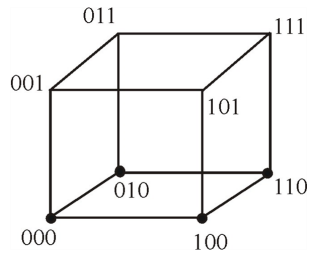
\includegraphics[width=2in]{images/p2.png}\\
	Figure 3: Boolean cube of dimension 3
\end{figure} 

\begin{enumerate}
  \item Compute the eigenvalues and eigenvectors of $B_n$.
    
  \Answer

  Let $Q_n$ be the adjacency matrix of $B_n$. We use $\lambda$ to denote the eigenvalues of $Q_n$.
  
  When $n = 1$, we have:

  \begin{equation}
    Q_1=\begin{bmatrix}
    0 & 1 \\
    1 & 0 \\
    \end{bmatrix}
  \end{equation}
  
  And we can get $\lambda=1,-1$.
  
  When $n = 2$, we have:

  \begin{equation}
    Q_2=\begin{bmatrix}
    0 & 1 & 1 & 0 \\
    1 & 0 & 0 & 1 \\
    1 & 0 & 0 & 1 \\
    0 & 1 & 1 & 0 \\
    \end{bmatrix}
    =\begin{bmatrix}
    Q_1 & I \\
    I & Q_1 \\
    \end{bmatrix}
  \end{equation}

  Therefore, $\lambda=-2,0,0,2$.
  
  When $n = 3$, we have:

  \begin{equation}
    Q_3=\begin{bmatrix}
    Q_2 & I \\
    I & Q_2 \\
    \end{bmatrix}
  \end{equation}

  And $\lambda=-3, -1, -1, -1, 1, 1, 1, 3$.
  
  We can conclude that

  \begin{equation}
    Q_n=\begin{bmatrix}
    Q_{n-1} & I \\
    I & Q_{n-1} \\
    \end{bmatrix}
  \end{equation}

  and the eigenvalues:
  $\lambda=-n,-n+2,-n+4,...,n-4,n-2,n$ with multiplicity
  $\binom{n}{0}$,$\binom{n}{1}$,\\$\binom{n}{2}$,...,$\binom{n}{n-2}$,$\binom{n}{n-1}$,$\binom{n}{n}$, respectively.
  The number of eigenvalues is $2^n$.

	\item Consider lazy random walk where we stay at the current vertex with probability .5 and move along an edge with probability .5. Bound the mixing time of lazy random walk in	$B_n$ by eigenvalues.
	
  \Answer
  We first consider the random walk.
	Let $A$ be the transition matrix of random walk of $B_n$ and $A = 1 \cdot Q_n$. We use $\eta$ to denote the eigenvalues of $A$ where $\eta_i = \frac{1}{n} \cdot \lambda_i$. From the lecture we have $\pi(j)=\frac{d(j)}{|E|}= \frac{n}{n \cdot 2^n}=\frac{1}{2^n}$.

  Then we consider the lazy random walk. Similar to above, the transition matrix of the lazy random walk is $A= \frac{1}{2} \cdot I + \frac{1}{2} \cdot A$. We use $\mu$ to denote its eigenvalues, where $\mu_i = \frac{1}{2} + \frac{1}{2} \cdot \mu_i =\frac{1}{2} + \frac{1}{2 \cdot n}\lambda_i$. From (1), we can obtain $\lambda \in [-n, n]$, so we have:

  \begin{equation}
    1 = \mu_1 \geq \dots \geq \mu_{2^n} \geq 0
  \end{equation}
  
  Let $v$ denote the eigenvectors of $A$. We have:

  \begin{align}
    v_1 &= (\sqrt{\frac{d(1)}{2m}}, \dots, \sqrt{\frac{d(n)}{2m}})^T \notag \\
    &=(\sqrt{\frac{1}{2^n}}, \dots, \sqrt{\frac{1}{2^n}})^T
  \end{align}

  Since $A$ is symmetric:

  \begin{align}
    A = \sum\limits_{i=1}^{2^n} \mu_i \cdot \overrightarrow{v_i} \cdot \overrightarrow{v_i}^T
  \end{align}

  
  \begin{align}
    p_t^T &= p_0^T \cdot A^t \notag \\
    &= p_0^T \cdot \sum\limits_{i=1}^{2^n} \mu_i^t \cdot \overrightarrow{v_i} \cdot \overrightarrow{v_i}^T
  \end{align}

  \begin{align}
    p_t(j) &= \sum\limits_{i=1}^{2^n} p_0(i) \cdot A^t(i,j) \notag \\
    &= \sum\limits_{i=1}^{2^n} p_0(i) \cdot [\pi(i)+ \sum\limits_{k=2}^{2^n}\mu_k^t \cdot v_k(i) \cdot v_k(j)] \notag \\
    &= \pi(j)+\sum_{i=1}^{2^n} p_0(i) \cdot [\sum\limits_{k=2}^{2^n}\mu_k^t \cdot v_k(i) \cdot v_k(j)]
  \end{align}

  \begin{align}
    ||p_t-\pi||_{1} &= \sum\limits_{j=1}^{2^n} |p_t(j) - \pi(j)| \notag \\
    &= \sum\limits_{i=1}^{2^n} |\sum\limits_{j=1}^{2^n} (p_0(i) \cdot \sum\limits_{k=2}^{2^n} \mu_k^t \cdot v_k(i) \cdot v_k(j) | \notag \\
    &\leq \sum\limits_{j=1}^{2^n} |2^n \cdot \max\limits_{k=2 \backsim 2^n} \mu_k^t| \notag \\
    & \leq 2^{2n} \cdot |\mu_2^t |
  \end{align}

  \item Argue that it takes $\Omega(n\log n)$ time to mix in expectation.
  
  \Answer

  Let $t \geq \frac{n \cdot \log n}{1-\mu_2}$, we have:

 \begin{equation}
 \begin{aligned}
    {||p_t-\pi ||}_1 & \leq 2^{2 n} \cdot |\mu_2^t| \\
  & \leq 2^{2 n} \cdot e^{-n \cdot \log n} \\
  &=\left(\frac{4}{n}\right)^n
 \end{aligned}
 \end{equation}

 So it takes $\Omega(n \log n)$ time to mix in expectation.

\end{enumerate}
\end{document}
